\begin{appendix}

\chapter{DMA Detailed Description}
\label{app:DMA-arch}
This appendix contains additional details about the DMA implementation, and serves to give a deeper understanding of how each component in the DMA works in details..
\section{DMA Architecture in details}
\subsection{Topview}
Figure \ref{fig:TopViewFinalSimple2IO} shows the entire DMA Module, with its components, \todo{Describe briefly inputs and outputs} inputs and outputs.


\begin{figure}[h!]
    \centering
    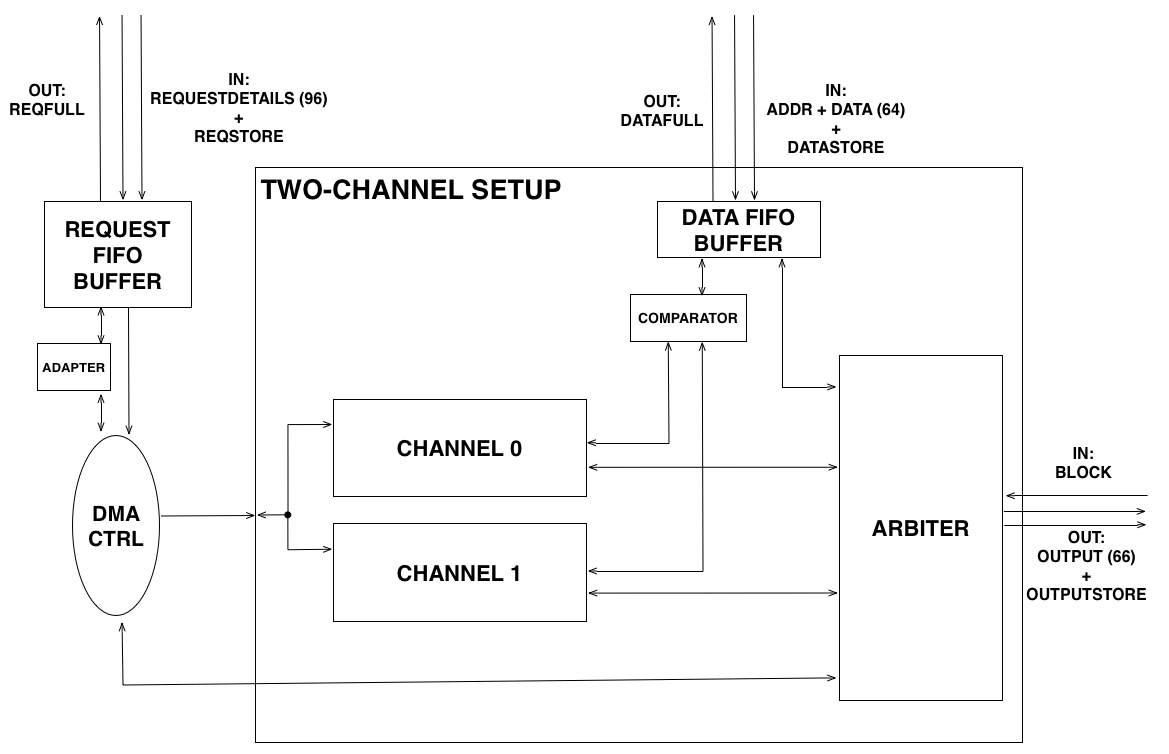
\includegraphics[width=1.0\textwidth]{Figures/DMA/TopViewFinalSimple2IO}
    \caption{Topview of the DMA Module, with its inputs and outputs}
    \label{fig:TopViewFinalSimple2IO}
\end{figure}

\subsubsection{Components}
These are the components that the DMA Module consists of:

\begin{description}
    \item[DMA Controller -] 
    The controlling unit responsible for handling transfer requests, monitor channel activity and sending out interrupt signals.
    \item[Channels -] 
    A channel is capable of performing a requested transfer, by issuing loads and stores.
    The system currently implements two channels.
    Each channel is split into two sub-modules, called "load channel" and "store channel"
    \item[Arbiter -]
    Used to select next output: Interrupt, store or load command.     
    \item[FIFO Buffers -]
    Two FIFO buffers are used to store transfer requests and data.
    \item[Comparator -]
    Used to identify which channel has requested the next data.
    \item[Adapter -]
    Used between Request FIFO buffer and the DMA Controller for proper synchronization between their signals.  
\end{description}

\subsubsection{Inputs and outputs}
Inputs and outputs for the entire Topview are mainly grouped by the FIFO buffers and the Arbiter.
\begin{description}
    \item[Request FIFO Buffer -] 
    The inputs are a control signal for storing in the FIFO buffer, and details on 96 bits: 32 for source address, 32 for destination address, and 32 for transfer details, including ID-number on the requesting peripheral and the count number. 
    \todo{Meh...}Not all bits from the transfer details are currently in use.
    The output signal is a FIFO full-signal, signaling that the buffer is full.
    \item[Data FIFO Buffer -] 
    The inputs are a control signal for storing, and data details on 64 bits: 32 for address of origin, and 32 for the data itself.
    The output signal is a FIFO full-signal, signaling that the buffer is full.
    \item[Arbiter -]
    The outputs that passes are a control signal to be used externally, and details on 66 bits: 2 first bits are used to identify the type of command, the rest are the details (interrupt, or load/store with address and data).
    The input block-signal may be used by the external system to pause the DMA module from sending out any more data, in case the external system is saturated and must process the current output before receiving any more. 
    The impact of this depends on the external system.
\end{description}

\subsection{DMA Controller State Machine}

The DMA Controller is implemented as a state machine.
It is responsible for handling requests to do data transfers, monitoring active channels, and sending out interrupt signal when a channel has completed its data transfer.
The state machine can be seen in figure \ref{fig:DMAControllerStateMachine}.

\begin{figure}[htb]
    \centering
    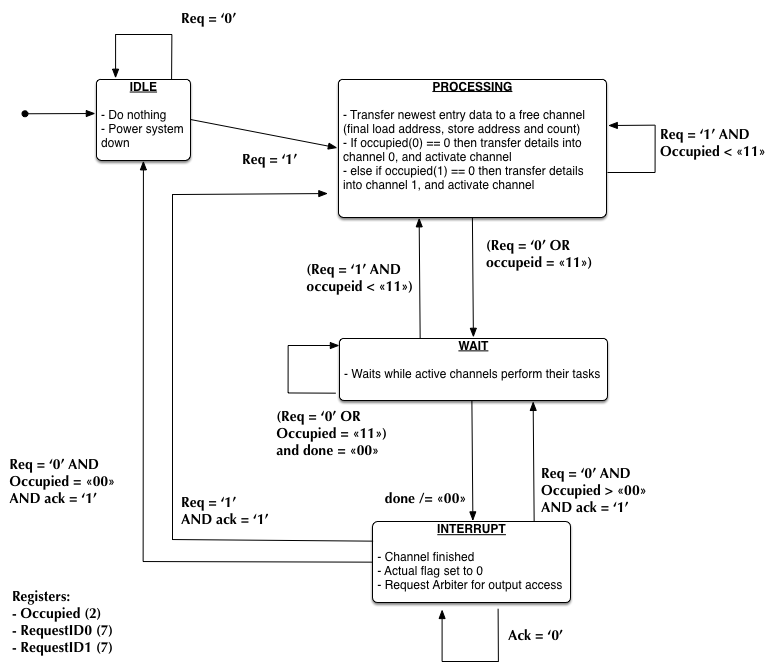
\includegraphics[width=1\textwidth]{Figures/DMA/StateMachineFinal}
    \caption{Detailed DMA Controller State Machine}
    \label{fig:DMAControllerStateMachine}
\end{figure}

\subsubsection{States}
The states used in the state machine are IDLE, PROCESSING, WAIT AND INTERRUPT

\begin{description}
    \item[IDLE -] 
    When there are no requests for data transfer.
    The DMA Controller waits until a request signal is received.
    \item[PROCESSING -] 
    When the controller has received a request, and there is a free channel to execute the request.
    Outputs from the DMA Main controller to a free channel is transfered, activating the channel.
    \item[WAIT -]
    When both channels are active and there are no more room for new requests to be processed, or when there are no more requests to process while there are still channels active.
    \item [INTERRUPT -]
    When a channel is finished with execution and no longer active, the DMA Main Controller will request the arbiter to send out interrupt request.
    Until the arbiter acknowledges the request, the controller will remain in this state, and no new requests will be processed until done.
    When acknowledged, the controller will send out an interrupt signal with necessary details, such as the ID of the requestor.  
\end{description}

\subsubsection{Inputs}
The DMA controller have the following inputs:

\begin{description}
    \item[clk -]
    Input clock signal
    \item[reset -]
    Reset signal that reverts state machine back to idle
    \item[req -]
    Input request signal for transferring data.
    \item[loadDetails -]
    The beginning 32-bit loading address
    \item[storeDetails -]
    The beginning 32-bit storing address
    \item[reqDetails -]
    32-bit details relevant for the transfer.
    Contains count, which is used for both offset and counting down the execution to finish, and ID-number of the requestor, which is used in the interrupt signal.
    \item[activeCh0 -]
    Monitoring signal from channel 0, signalizing that it is currently active.
    \item[activeCh1 -]
    Same as activeCh0, but for channel 1.
    \item[interruptAck -]
    Signal from arbiter that the DMA Controller has access to send out interrupt signal from the system.
\end{description}

\subsubsection{Outputs}
These are the following output signals from the DMA controller

\begin{description}
    \item [reqUpdate -]
    Signal to acknowledge the received data transfer request (req) and its details, so that next request may be received.
    Used in facilitating pop-signals at the Request FIFO buffer.
    \item[FLAOut -]
    32-bit FLA (Final Load Address) output sent to channels.
    Calculated by adding loadDetails with count.
    \item[FSAOut -]
    32-bit FSA (Final Store Address) output sent to channels.
    Calculated by adding storeDetails with count.
    \item[counterOut -]
    32-bit counter output sent to channels.
    \item[set0 -]
    Signal used to activate channel 0 and store FLA, FSA and counter data to it.
    \item[set1 -]
    Same as set0, but for channel 1.
    \item[interruptReq -]
    Request signal to the arbiter for sending out interrupt
    \item[interruptDetails -]
    34-bit interrupt details, sent out of the DMA Topmodule when the controller requests the arbiter for access, and is acknowledged.
    Contains 2 bits to recognize interrupt with values are 11, and contains ID of the transfer requestor. 
    These make up 7 bits. 
    The other bits are currently not in use.
\end{description}

\subsubsection{Internal registers and signals}
The DMA controller also has some internal registers and signals.
These are:

\begin{description}
    \item[occupied -]
    A 2-bit register, with each bit representing a channel each.
    When the DMA controller activates a channel, it also sets the corresponding bit in the occupied-register to '1'.
    The occupied-register is compared with the incoming active-signals from the channels.
    Whenever a channel finishes and deactivates, there is a difference bewteen the active signals and the occupied-register, and the controller compares the values and the active signals to determine which channel has finished.
    \item[requestID0 -]
    A 7-bit register, containing the ID of the requestor of the transfer currently being executed in channel 0.
    The ID is included in the interrupt signal the DMA controller sends out when the transfer is done executing in channel 0.
    \item[requestID1 -]
    Same as RequestID0, but for channel 1.
    \item[totalActive -]
    A 2-bit signal, which is the concatination of both the active signals from the channels.
    The DMA Controller needs the active signals immediately when set-signals are sent out to function properly, yet there is a cycle delay from the current channel setup.
    Therefore the setX-signals are also checked when totalActive is set.
    This is done by using setX OR activeX.
    \item[workDone - ]
    This is the signal used to determine whether a channel is done executing or not.
    workDone is calculated by subtracting the values of the occupied-register with the values of the totalActive signal.
    If the value is not "00", then a channel has finished, and the controller enters an interrupt state.
    The occupied-register is updated as well.
\end{description}

\subsection{DMA Request FIFO adapter}

The DMA Controller is designed to prosess input data that arrives together with the request signal, but the FIFO design that is used to store requests is not fully compatible with this setting.
The reason they are not compatible can be explained by using an example where only one request has been stored into the FIFO buffer.
When content is stored, the empty-signal from the FIFO buffer is set from '1' to '0'.
This is the only signal that is depenendant on whether there is content or not, and should thus be used as request signal.
However, when request is stored in the FIFO buffer, the new request is not automatically set as output.
For this to be done, the request must be popped.
When popped, the request data is set to the output, and the DMA controller receives it.
But since there are no other requests stored and waiting to be processed, the FIFO buffer will count as empty, and the empty signal is set to '1' (negating any request signal into the controller).
In summary, the problem is this: Either the controller will receive old data from a previous request with when new request, or there will be no request signal with the new data.
This is the case when there are only 1 request.
For a series of requests, the first request signal will be coupled with old data, while the final request will not be processed.
A further problem is to avoid having the controller popping wrong at in the FIFO buffer.
When a pop occurs, the FIFO buffer changes output by one \todo{sounds stupid, improve} storing cell, and it is possible to do a pop, even if the empty signal is '1'.
The empty signal is based on whether the FIFO's top and bottom have the same index, with pop as last command, and popping moves the bottom index.
Popping wrong will therefore create a wrong empty signal, and when processing the final request, the DMA Controller must not pop wrongly.

\par
The challenge is to make sure that request signals arrives at the same time with the corresponding data, and to make sure that incorrect pops to not occur.
Here is where the adapter comes in.
The adapter is designed to interface between the request FIFO Buffer, and the DMA Controller. 
It delays the request signals from the FIFO buffer by one clock cycles, and sends out pop-signals at correct time.
Figure \ref{fig:adapter} shows how the adapter is built up, and also how the adapter, the FIFO Buffer and the DMA controller are all connected to each other.


\begin{figure}[h!]
    \centering
    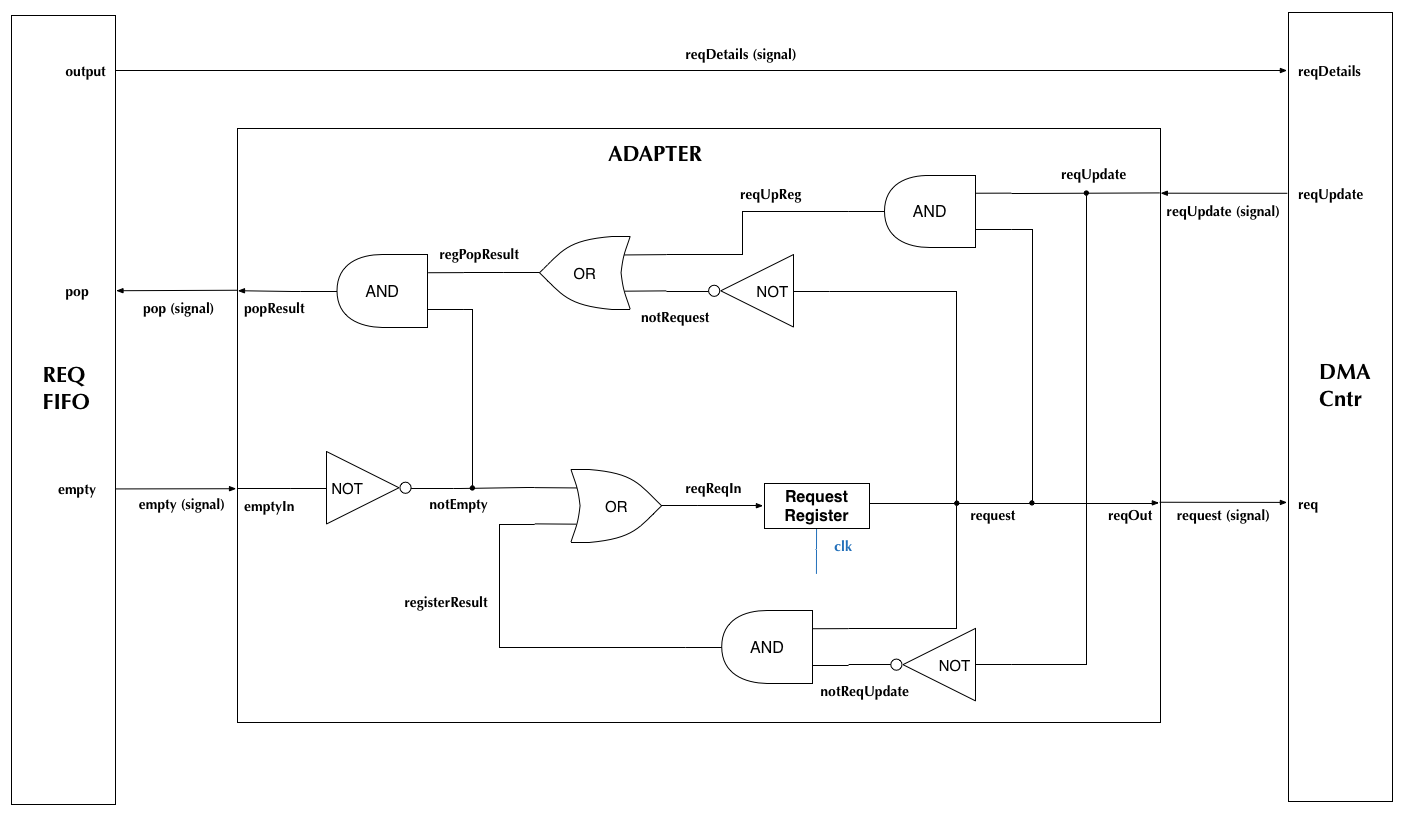
\includegraphics[width=1.0\textwidth]{Figures/DMA/Adapter}
    \caption{Adapter between FIFO Buffer and DMA Controller}
    \label{fig:adapter}
\end{figure}

The adapter has one register for storing request signals, but otherwise consists of combinatorics.
When a request is stored in the FIFO buffer, and the empty signal is sent in and negated, if the current value of the request register is 0, then the request is the first to arrive, either alone or in a series of requests.
The adapter pops the FIFO buffer, and the request data is stored in the register (NOT empty AND NOT request).
The register sends out the request the next cycle, which arrives in the DMA Controller together with the newly popped data.
As long as there are more in the FIFO buffer, the negated empty signals combined with the reqUpdate-signal from the DMA controller is used to pop for new requests (NOT empty AND (REQUEST AND reqUpdate).
ReqUpdate is set immediatly inside the DMA Controller whenever it receives a request and has a free channel.
When a request is processed, the next request details is popped at the same, so that they may be ready for input reading.
Using a register, any request signals are delayed with at least one cycle, so that output details from the FIFO buffer is popped and reaches the DMA Controller together with the corresponding request signal.
There are, however, some more issues to be aware of:
When the final data has been popped, the negated empty-signal becomes '0', but the expected case will be that while final data is ready to be read, there are no free channels to process the final request for a while.
The request register must store the final request, without being overwritten by the empty-signal.
This is done by using it's own value to update itself, until the next reqUpdate-signal is sent out, signaling that the DMA Controller has processed the final job.
As long as there is no more requests, and the negated empty-signal is '0', the request register will be set to '0' as well when the reqUpdate signal is sent out.
Notice also that as long as the negated empty-signal is '0', no pops will be made to the FIFO buffer either. 

\subsection{Manual subtractor}
One of the main components used inside both load channels and store channel is the manual subtractor.
It works by taking three inputs, two for subtraction and one as control signal.
If the control signal is active, the first input will have its value subtracted by the second input, and the output is the result.
If the control signal is not active, there will be no subtraction, and the first input value is the output value. 

\subsection{Load channel}
The load channel is responsible for generating loading requests that are sent out from the DMA.
It can be seen in figure \ref{fig:loadChannel}.

\begin{figure}[h!]
    \centering
    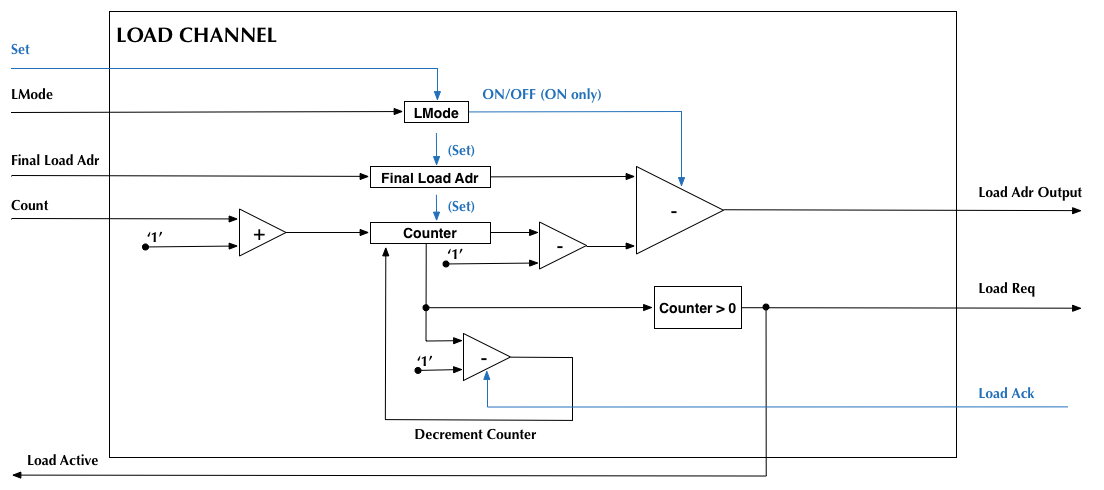
\includegraphics[width=1.0\textwidth]{Figures/DMA/LoadChannel}
    \caption{Load Channel}
    \label{fig:loadChannel}
\end{figure}

\subsubsection{Inputs}
The load channel have the following inputs:

\begin{description}
    \item[clk -]
    Input clock signal
    \item[reset -]
    Reset signal that clears all 
    \item[set - ]
    Signal from DMA Controller used to set all registers to the input values
    \item[LMode -]
    Value for LMode register
    \item[FLA -]
    32-bit value for the FLA register
    \item[Count -]
    32-bit value for the Counter register
    \item[Load Ack -]
    Signal received from the arbiter, telling that the current load request is acknowledged.
\end{description}

\subsubsection{Registers}
The load channel have the following registers:

\begin{description}
    \item[LMode -]
    Register for loading mode, connected to the subtractor.
    \item[FLA -]
    Contains Final Load address
    \item[Counter -]
    Used to count down the number of load requests to be generated. Also used to calculate offset from FLA, if LMode = '1'.
\end{description}

\subsubsection{Outputs}
The load channel have the following outputs:

\begin{description}
    \item[Load Adr Output -]
    34 bit signal with the address for the current load command. Is concatenated with two bits with value "00", used as MSB.
    \item[Load Req -]
    Request signal from the load channel to the arbiter, for requesting output access to issue load command to the system.   
    \item[Load Active -]
    Signal sent out, used to indicate that the load channel is active.
\end{description}

With exception from Load Ack from the arbiter, all input signals are received from the DMA Main Controller.
When set is active, all registers are overwritten by the matching input signals.
LMode determines if the loading requests are for a fixed address, or a block of addresses, by activating or deactivating a manual subtractor that the FLA and the Counter are connected to.
If LMode is active, the current load address is calculated by subtracting the FLA with the current counter value (minus 1).
Counter is used for both offset calculation, and counting down the number of remaining requests.
A unique number is needed to identify whether the current job is done or not, and the value 0 has been chosen for that.
As long as counter has a value above 0, the job is not done, and both load request and load active signals are active.
The Load Channel does not need any additional data or input signals beside the registers, therefore the channel is designed to issue loads as long as counter is not 0.
At the final count, the final load address should be issued, but if the counter value is 0, there will be no requests.
This is avoided by incrementing the Count input value by one when issuing a new job (set = '1'), and decrementing the counter's current value by one before subtracting with FLA.
Thus, when issuing the final load, the counter's value is "...001" while the counter's output value to the manual subtractor is 0.
The load channel can issue the final load, and then the counter reaches 0 when done.
The counter is also connected to another manual subtractor, which decrements the value with 1 if activated.
Except from when the set-signal is active, the counter is always overwritten by the result from this subtractor.
This manual subtractor is activated by the load ack-signal from the arbiter.
Whenever the lod ack signal is active, the current load address output passes through the arbiter, and the counter is decremented by one.

\subsubsection{Why final loading address, and counting down the offset?}
When designing the load channel, the needs were at least a static address for loading, an offset from that address, and a value for counting down the remaning loads to be issued.
The needs are the same for the store channel as well.
The current design incorperates both offset and counting into one single register.
The current address can be calculated by having a starting address that is added together with a current offset.
Alternatively, one may use a final address and subtract it with the offset.
If counting down, the zero-value is distinguishable from non-zero values, and can be used to know whether countdown is finished or not.
If a counter has an increasing value, there must be an extra register that contains the final count value so that the load channel can know when the job is finished.
In order to utulize as few registers as possible for the task, the counter and offset value has been joined as one register, and the system counts down towards zero.
This eliminates the need for any extra final count-register, since the counter can be checked for zero or non-zero values.
This means also using the final load address and subtracting it with the offset-value from the counter, when calculating current address.
\todo{Find a suitable place for this description}

\subsection{Store channel}
The store channel is responsible for generating storing requests, together with the correct data that has been loaded from a distinct memory address into the DMA module.
It can be seen in figure \ref{fig:storeChannel}.


\begin{figure}[h!]
    \centering
    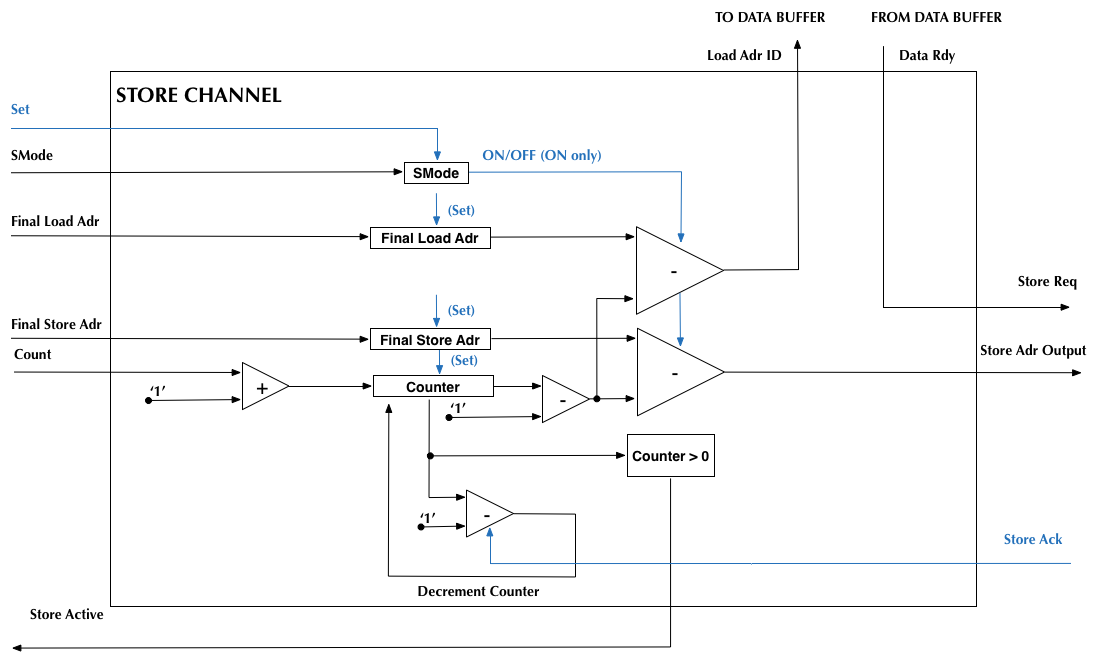
\includegraphics[width=1.0\textwidth]{Figures/DMA/StoreChannel}
    \caption{Store Channel}
    \label{fig:storeChannel}
\end{figure}

\todo{Consider if listing up inputs and outputs that are also found in the Load Channel is necessary}
The design of the store channel have similar traits to the load channel, and inputs, registers and outputs to the store channel, which can be seen in figure \ref{fig:storeChannel}, are similar to the ones from the load channel.
There are some distinct differences to know of:
\begin{description}
    \item[FSA and FLA -]
    There are both inputs and registers for the Final loading address and the final storing address.
    \item[Unique inputs and outputs -]
    Not similarly found in the load channel.
    These are the input data rdy, and the output Load Adr ID.
    \item[Store req -]
    Request signal from the store channel to the arbiter is not based on the counter, but on the input data ready.
\end{description}

Any loads issued by the load channel cooperating with the store channel is expected to reach a data buffer shared by all channels.
All received data has an ID, informing which address in the memory the data was loaded from.
Load Address ID, based on the FLA decremented with the counter, is compared with the ID of the next data in the buffer.
If there is a match, the next data belongs to this channel, and a data rdy-signal is sent in.
In this design of the store channel, the data rdy is used as request signal.
\todo{Is this said well enough?}
The reason behind this design is due to treating the Store Channel as a black box from outside, so that the if the store channel is replaced or changed in the future, the outside world does not need to know anything of it.
Since there is a corresponding storing address for every loading address, the counter is used to calculate offsets from both FLA and FSA.
Notice that there is no data sent into the store channel.
The data is provided by a shared data buffer, and sent straight through the arbiter.
The store channel sends out the storing address, together with two bits for storing commands.
These two bits are concatenated with the address, and are the two MSBs, with values "01".

\subsection{Arbiter}
The arbiter is used to arbitrate between all channels and the DMA Main controller, when any has \todo{Sounds stupid}outputs to send out of the system.
For each clock cycle, it selects between a number of requests, and allows selected command and data to pass through.
It can be seen in figure \ref{fig:arbiter}

\begin{figure}[h!]
    \centering
    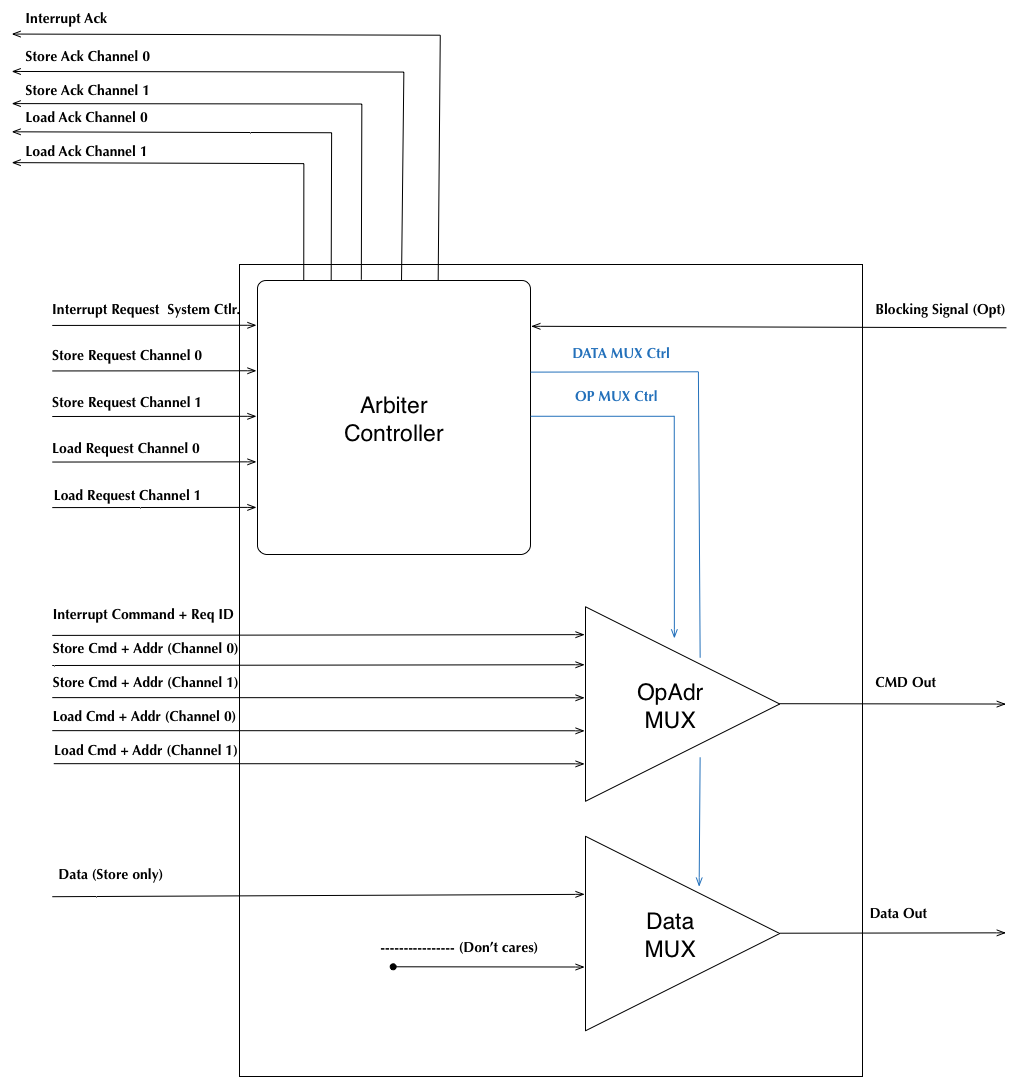
\includegraphics[width=1.0\textwidth]{Figures/DMA/Arbiter}
    \caption{Store Channel}
    \label{fig:arbiter}
\end{figure}

The arbiter receives store request and load request signals from each channel, as well as an interrupt request from the DMA Main Controller.
Each channel receives one store acknowledge signal and one load acknowledge signal from the arbiter.
The DMA Main Controller also receives interrupt acknowledge signal from the arbiter.
For each channel, there are two 34-bit command inputs, one for storing requests and one for loading requests.
There is also a 34-bit interrupt input from the DMA Main Controller.
All these command requests go through a 34-bit multiplexer, set by the Arbiter Controller, based on which request is acknowledged.
For instance, if a storing request from channel 1 is selected, the store details from channel 1 is the one that passes through the multiplexer and reaches CMD out.
The data input comes from the shared data buffer, and is sent through the Data Multiplexer whenever there is a storing request that is acknowledged.
There is also a blocking signal connected to the arbiter.
If the blocking signal is active, then no requests will be acknowledges, and any work inside the DMA Module, whether it's a channel or the DMA Main Controller, will effectively be halted.
The system bus is expected to be the bottle neck in this design, and any outputs from the DMA Modul must not be sent out faster than the system can handle.
Should there be any need, the system needs to be able to halt the DMA Modul in issuing any more commands until the previous command(s) can be handled. 

The priority from the Arbiter Controller is:
\begin{itemize}
    \item Block, then intterupt, then stores, then loads
    \item If there are two stores or two loads competing, then the least recently used channel gets priority.
    This way the commands sent out from the DMA Module will alternate between two active channels. 
    This is separate for load requests and store requests.
\end{itemize}

\subsection{Comparator}
The comparator is used to compare the current output data's loading ID with the loading ID the requesting store channels are waiting for.
The channel that has a match receieves a data rdy signal from the comparator. 

\subsection{FIFO Data buffer}
The implemented data buffer is a FIFO buffer.
It is 64 bits wide, 32 bits containing the address from where the data is loaded, known as LoadID, and 32 bits containing data itself.
\todo{Write a bit more, about purpose and reasonable depth} 

\subsection{Interaction in the two-channel setup}
The channels are set up in a sub-module of the DMA Module, called the TwoChannelSetUpBuffered.
This setup can be seen in figure \ref{fig:twoChannelSetup}.
The figure shows how two channels 0 and 1 are combined in this submodule together with FIFO data buffer, a comparator, and an arbiter.

\begin{figure}[h!]
    \centering
    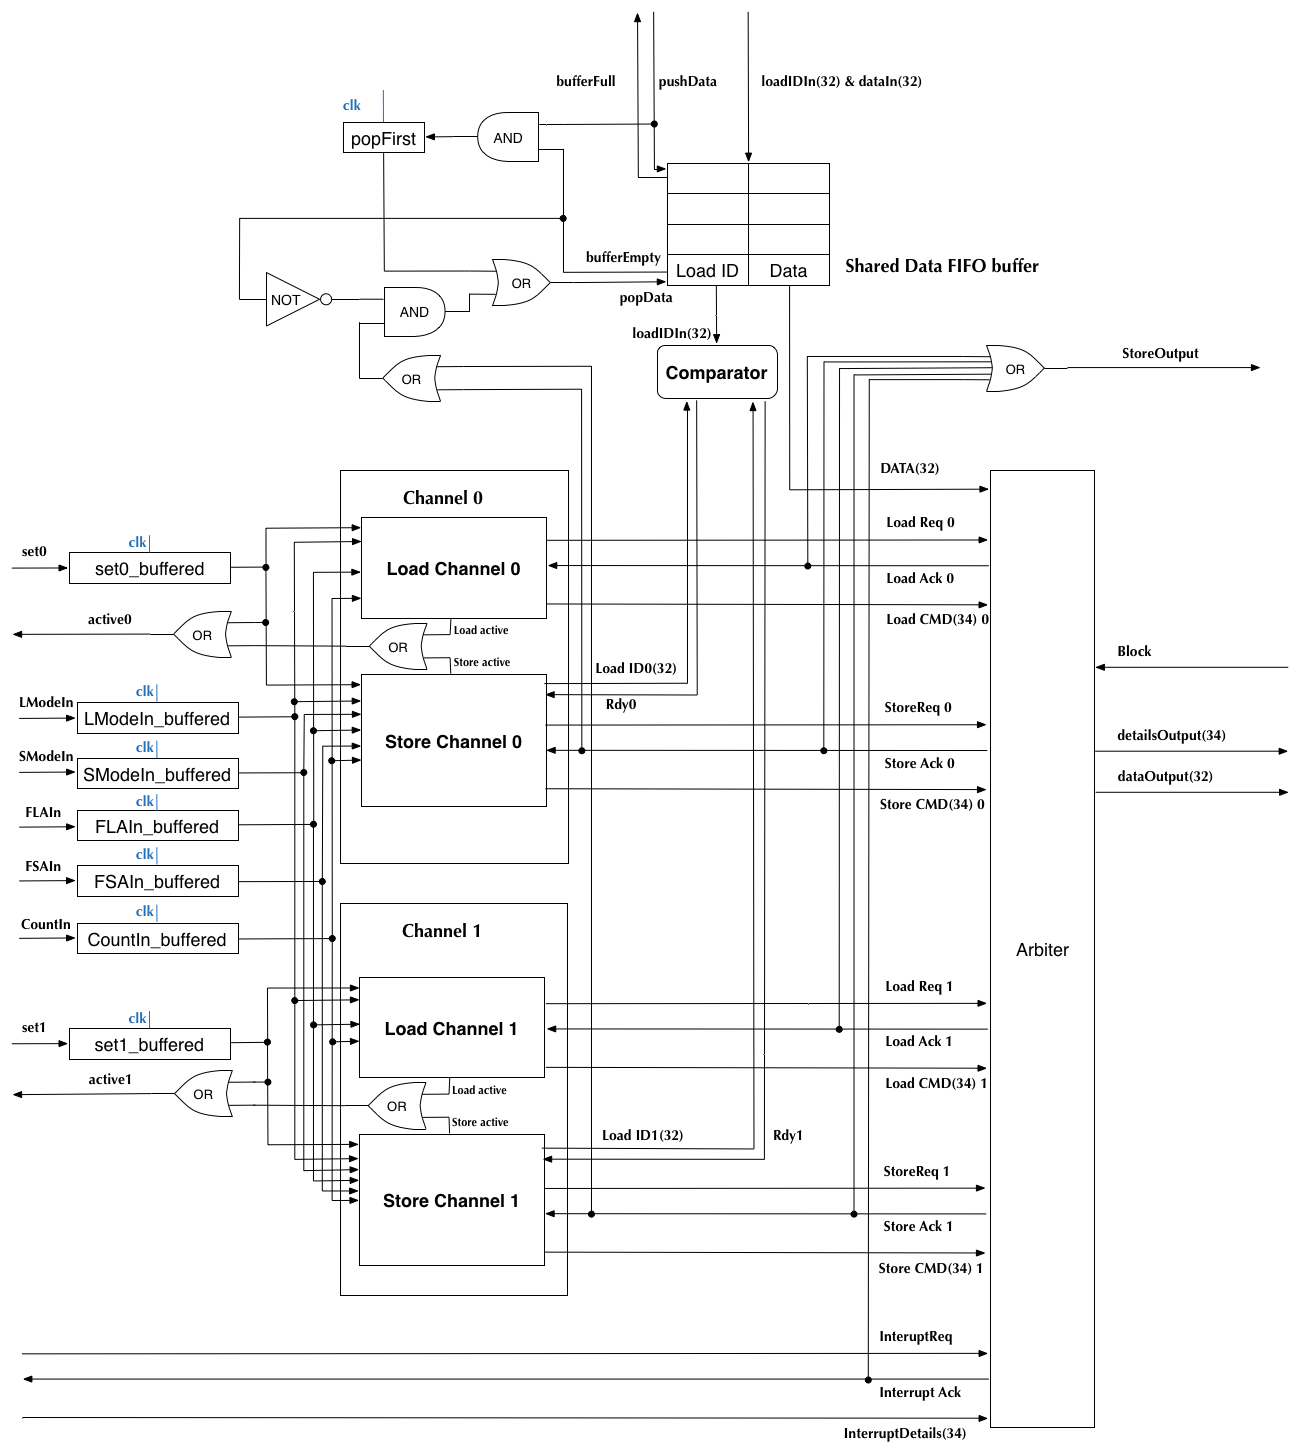
\includegraphics[width=1.25\textwidth]{Figures/DMA/TwoChannelSetUpBuffered}
    \caption{The two-channel setup, buffered version}
    \label{fig:twoChannelSetup}
\end{figure}

The choice of designing a submodule with the channels, was mainly to have a working environment where testing the interaction between the channels, arbiter and input buffer, were possible before having finished the DMA Main Controller.

All inputs to the channels from the DMA Controller go through synchronous buffers.
Originally, the setup were originally designed without buffers, but behavioral simulation showed that whenever a set-signal was received exactly at a clock tick together with new inputs, the previous counter value would be written into the counter registers in the channels.
The rest of the inputs to the channels were correctly written.
The counters are the only registers which inputs must pass additional combinatorics, so apparently these values did not reach the counter registers in time with the set-signal.
Adding buffers for all input signals solved this problem, by giving all inputs to the channels an entire cycle to synchronize.
The cost is an additional cycle in activating the channels.

The DMA Main controller, which sends in these inputs, is also connected directly to the arbiter.
Whenever the DMA Main Controller needs to send interrupt signals, this goes through the arbiter.

Notice that each set\_buffered registers are also connected to the respecite active-signal that are sent back to the DMA Main controller.
Even if buffering the inputs delays the channel activation by one cycle, the DMA Main controller should still receive the active-signal as early as possible.

\todo{Remember, you have a design flaw to fix. Update figure and text when it is done}
Popping data from the data buffer at the right time is also a challenge.
Whenever a channel stores the lates data from the FIFO buffer, new data should be popped, but only if there is more.
If the buffer is empty, no more pops should be issued.
Whenever new data arrives to an empty buffer, it must be popped first before any of the channels can read the ID.
This is solved by implementing some combinatorics, and a register called popFirst.
When new data arrives, there must be a cycle between the push and the pop.
popFirst is set by combining the empty-signal with the push-signal, which are both active when the first data arrives, and popFirst will be used in popping the first data during the next cycle.
Otherwise, if there is content in the buffer that is to be popped, it will be done so as long as the empty signal is low, and as long as any of the store ack-signals from the arbiter is active (meaning that data with storing address is sent through and out of the DMA Module).

Whenever something is sent through the system, either a store request, load request, or interrupt, an additional signal StoreOutput, is sent.
This is done by combining all ack\-signals into an OR gate, named StoreOutput.
This is to be used as a separate signal to the system that handles outputs from the DMA Module, to signal that a new output is sent out.
Suppose there is a loading request sent out to address 0.
\todo{Probably first mention of command value 00, should find a place where the values 00, 01 and 11 are described}
The command is then "00", and the address consists of 32 0's.
The receiving output system would not know the difference between this load, and an inactive module (default are 0's).
Using a separate signal solves this issue.

\subsection{Tweaks in the system}
\todo{Meh.... But mention in end of main report that these tweaks must be replaced with proper solution}
The DMA module was designed for word addressing, while the system used to test the hashing module and the DMA module in this project uses byte-addressing.
The current design does not support both, and in order to both save time and adapt the DMA module to the test system, these changes were done:
\begin{itemize}
    \item The DMA Controller multiplies the counter value with 4 before calculating FLA and FSA
    \item The multiplied countervalue is stored in the channels
    \item The channels decrement with 4 instead of 1 
\end{itemize}

\section{Verification and testing of DMA Module}

%\section{Functional testing}
The DMA Module is tested by first testing individual components, then their interaction with each other.

In the individual testing, the component receives different combinations of the inputs as the time passes.
The test shows whether the component behaves as expected, based on the input.
This is done by reading the outputs based on inputs and/or values of internal registers.
Components that are tested individually are:
\begin{itemize}
    \item \textbf{Adapter} 
    \item \textbf{Arbiter Controller}
    \item \textbf{DMA Main Controller}
    \item \textbf{Load Channel}
    \item \textbf{Store Channel}
\end{itemize}

In the interaction testing, also known as topview-testing, the components are tested for their interaction with each other.
Since the components have been tested individually, they are assumed at this point to be functional. 
Internal values are thus ignored, also since the focus of the tests are to ensure that the interaction between the components are working as expected.
The interaction tests are:
\begin{description}
    \item[Arbiter -]
    Tests that internal multiplexers are set correctly by the controller, based on the selected requests.
    \item[Two Channel setup, signle request -]
    First of two tests that checks if the two-channel setup works as expected, by activating a single channel.
    Data with ID is fed manually to the data buffer.
    The tests ensures that a load channel sends out number of requests according to count value, and that whenever data arrives, stores are issued and get priority above loads.
    Also tests if interrupts and blocks get highest priority, and that active signals are activated and deactivated correctly.
    \todo{This is actually just saying that I didn't add separate counters here as I did in the topview test for the entire module}
    Correctness is ensured by reading the output values (mainly detailsoutput and dataOutput) from the two-channel setup.
    \item[Two Channel setup, two requests -]
    Second of two tests, this one activates both channels.
    In addition to the first test, this one also ensures that loads from both channels alternates when both are active, and that correct channel identifies and stores the correct data that has been loaded.
    When one channel is done, the other channel will have full access to the arbiter, and loads will no longer alternate.
    Correctness is ensured by reading the output values. 
    \item[Two Channel setup, two requests -]
    Second of two tests, this one activates both channels.
    In addition to the first test, this one also ensures that loads from both channels alternates when both are active, and that correct channel identifies and stores the correct data that has been loaded.
    When one channel is done, the other channel will have full access to the arbiter, and loads will no longer alternate.
    Correctness is ensured by reading the output values.
    \item[Topview -]
    This is where the entire DMA Module is tested, as requests are sent in.
    Each cycle with load, store, interrupt and blocking are counted (either identified by the command value, or by the blocking signal when it is high, in the test).
    For each load issued, a register receives the load address, and sends it back to the DMA Module with a push signal and data (since the data value is not important for this test, each value is incremented by 8).
    Thus there is a cycle delay from a load is issued to the data arrives to the DMA Module.
    In the real world, there will be far more cycles from a load is issued, until it's data arrives in the DMA Module.
    And issuing multiple loads or not also depends on the system it is integrated with.
    There will be great difference between this project, where the DMA Module is connected to a single shared bus network, and to integrate it on SHMAC, where the main network is switched-media network.
    In this test, however, all data arrives quickly, as if using a bus and memory that is extremely fast.
    One reason is to cut down the necessary waiting time in the test itself, and another is that the module is tested for near-maximum peak.
    There are three tests in total: One with single request (only one channel active), one with two requests (both channels active) and one with four requests (test for waiting requests).
    Correctness is ensured by comparing the test counter values with expected number of loads, stores, interrupts issued, and number of blocks.
    
    \todo{HHHHHHMMMMMMM!!!!!}A word of warning: It turns out in the tests that for each round of blocks, the block counter counts one block less than the number of cycles a block is active. It still turns out, when analysing the signals, that the module is inactive in correct number of cycles as long as the block signal is active, the block counter merely does not count for the first cycle during a block. Since this is considered a flaw with the test itself, and not with the DMA Module, the error is considered negligable. 
\end{description}


\end{appendix}

